\section{Methodology}
\subsection{Personas}
Marketing communication applications have the quirk of having no direct impact of the targeted users on the product. They cannot directly be interviewed for goals and requirements. Additionally the group of targeted users is normaly to large to wrap your head around them. That is the reason for using personas. Human brains are caring more bout individuals, than large groups \parencite[cf.][]{Platt.2016}. Reasoning, archetypal individual people \parencite[cf.][81-82]{Cooper.2007}, which embody specific characteristics of groups \parencite[cf.][]{Platt.2016}. Identifying, analyzing, and prioritizing personas is a multistage procedure, which is always based on a type on research \parencite[cf.][39]{Robier.2016}. Research methods for this kind do not claim to scientifically acurate, but must not be based solely upon stereotypes and arbitrary decisions \parencite[cf.][82-83]{Cooper.2007}. 
\paragraph{} For identification of relevant stakeholders \textcite[38]{Robier.2016} suggest the usage of a stakeholder map (cf. \Cref{fig:stakeMap}). People of the left hand side of the vertical axis are the users of the program, divided into heavy users (far left) and fist time users (narrow to the axis) \parencite[cf.][38]{Robier.2016}. This approach aims not at the identification of each individual stakeholder, but at the identification of stakeholder groups to be represented by a persona \parencite[cf.][82]{Cooper.2007}, explicitly  including non-users \parencite[cf.][84]{Cooper.2007}.
\begin{figure}[H]
    \centering
    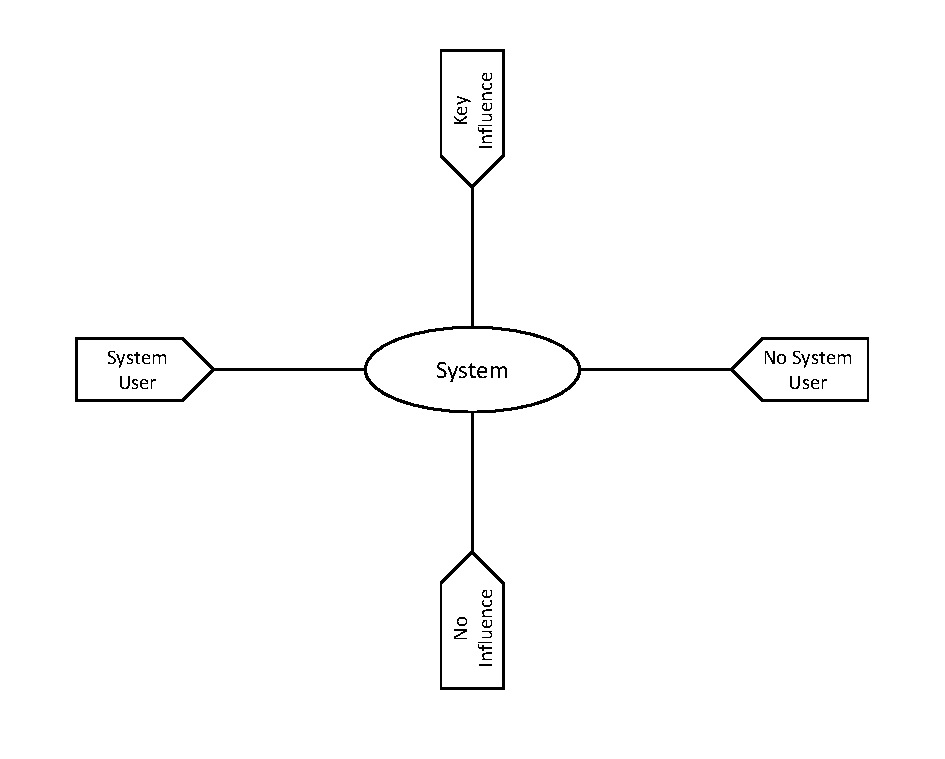
\includegraphics[scale=0.7]{img/stakeholderMap.pdf}
    \caption[Stakeholder Map]{Stakeholder Map (own illustration based on \cite[38]{Robier.2016})}
    \label{fig:stakeMap}
\end{figure}
Analysis of the personas identified, includes the specification of a personas traits. Since personas are represented as individual people \parencite[cf.][81]{Cooper.2007}, it has all attributes a natural person has, including a name, gender, age, family, education, and most importantly: a motivation \parencites[cf.][]{Platt.2016}[cf.][83-84]{Cooper.2007}. All traits of a persona must be contributing to a bigger picture, and thereby must be intentionally be set to suggest intended characteristics \parencite[cf.]{Platt.2016}. 
\paragraph{} As an example: Our persona Kevin Smith (25, male) works at a international bank as foreign trade manager after his studies in financial management at Harvard Business School and needs a way to plan his meetings in accordance to required travel times. In his free time he has a private single engine plane. If you ask yourself whether Kevin needs his schedule in a standardized time zone, such as UTC, the answer will definitely be yes, because he is on the one hand used to using UTC at work and in his hobby. Martha Jones (55, female) works at a local retailer since her diploma from community college, now being store manager, requiring a tool to plan and distribute shifts of her employees. She on the other hand will have more use for local time. Both may be personas for a calendar service focused on business customers. 
\paragraph{} All traits of Kevin and Martha will have implications on the conception and development of the hypothetical calendar service. Beside the very different functionality requests of transport service provider integration, respectively shift planning and public calendar provisioning, the age may have implications on the devices used, as well as the education implies different kinds of prior knowledge. 
\subsection{Natural Language Requirement Notation}
\subsection{Diagrams}
\subsection{Visual Design}